%%
%% licence       kaneton licence
%%
%% project       kaneton
%%
%% file          /home/mycure/kaneton/view/papers/assignments/assignments.tex
%%
%% created       julien quintard   [wed dec  7 16:53:52 2005]
%% updated       julien quintard   [fri mar  3 09:50:18 2006]
%%

%
% template
%

%
% ---------- header -----------------------------------------------------------
%
% project       kaneton
%
% license       kaneton
%
% file          /home/mycure/kaneton/view/template/paper.tex
%
% created       julien quintard   [wed may 16 18:17:37 2007]
% updated       julien quintard   [fri oct  5 07:00:45 2007]
%

%
% class
%

\documentclass[10pt,a4wide]{article}

%
% packages
%

\usepackage[english]{babel}
\usepackage[T1]{fontenc}
\usepackage{a4wide}
\usepackage{fancyheadings}
\usepackage{multicol}
\usepackage{indentfirst}
\usepackage{graphicx}
\usepackage{color}
\usepackage{xcolor}
\usepackage{verbatim}
\usepackage{aeguill}

\pagestyle{fancy}

\setlength{\footrulewidth}{0.3pt}
\setlength{\parindent}{0.3cm}
\setlength{\parskip}{2ex plus 0.5ex minus 0.2ex}

%
% logos
%

\newcommand{\logos}
  {
    \begin{center}
      
\includegraphics[scale=0.8]{\path/logo/kaneton.pdf}
    \end{center}
  }

%
% prototype
%

\newcommand\prototype[2]{
  \begin{tabular}{p{0.2cm}p{13.8cm}}
  & #1
  \end{tabular}

  \begin{tabular}{p{1cm}p{13cm}}
  & #2
  \end{tabular}}

%
% verbatim stuff
%

\definecolor{verbatimcolor}{rgb}{0.00,0.40,0.00}

\makeatletter

\renewcommand{\verbatim@font}
  {\ttfamily\footnotesize\selectfont}

\def\verbatim@processline{
  {\color{verbatimcolor}\the\verbatim@line}\par
}

\makeatother

%
% header
%

\rhead{}
\rfoot{\scriptsize{The kaneton microkernel project}}

\date{\scriptsize{\today}}


%
% header
%

\lhead{\scriptsize{The kaneton microkernel project assignments}}

%
% title
%

\title{The kaneton microkernel project assignments
       \logos}

%
% authors
%

\author{\small{Julien Quintard},
        \small{Matthieu Bucchianeri} and
        \small{Renaud Voltz}}

%
% prototype
%

\newcommand\prototype[1]{\hspace{1.5cm}#1}

%
% document
%

\begin{document}

%
% title
%

\maketitle

\newpage

\tableofcontents

\newpage

%
% --------- text --------------------------------------------------------------
%

%
% the project
%

\section{Overview}

To get more information about the kaneton project and the kaneton
microkernel reference, please take a look at the kaneton reference
document.

All the kaneton documents are available on the official website:
\textbf{http://www.kaneton.org}.

The present \textit{Assignments} document must be used by students
willing implement the kaneton microkernel design.

This document is under the \textbf{kaneton license}

%
% ---------- header -----------------------------------------------------------
%
% project       kaneton
%
% license       kaneton
%
% file          /home/mycure/kaneton/view/book/assignments/future/k0.tex
%
% created       julien quintard   [fri nov 28 05:25:37 2008]
% updated       julien quintard   [sat nov 29 16:07:29 2008]
%

%
% ---------- k0 ---------------------------------------------------------------
%

\chapter{k0}
\label{chapter:k0}

\name{k0} is an introduction to low-level programming.

\newpage

%
% ---------- text -------------------------------------------------------------
%

\section{Abstract}

k0 is an introduction to low level programming. During this first step of
the kaneton project, you will deal with:

\begin{enumerate}
  \item
    {\bf Intel x86}

    x86 assembly and architecture
  \item
    {\bf BIOS interrupts}

    How to use BIOS services
  \item
    {\bf ELF binaries}

    Structure and execution of an ELF file
\end{enumerate}

The final goal is to write a complete ELF bootloader, which could be used to
load a kernel.

\clearpage

%
% String display
%

\newpage

\section{Exercises}

\subsection{String display}

\subsubsection*{Overview}
In this first exercise you will learn how to use Video BIOS Services to
print strings on the screen.

\subsubsection*{Assignments}
The work is divided up into several steps. First, try to print a char and
to move the cursor on the screen and then, use those functions to display
a string.

\subsubsection*{File}
\begin{itemize}
  \item \location{ex1/ex1.S}
\end{itemize}

\subsubsection*{Interface}
\command{print\_char}
{
  Print the character which ASCII code is \argument{\%al} at current cursor
  position.
}

\command{cursor\_set}
{
  Set cursor position at row \argument{\%dh} and column \argument{\%dl}.
}

\command{print\_string}
{
  Print the string pointed by \argument{\%si} at row \argument{\%dh} and
  column \argument{\%dl}.
}

%
% Registers dump
%

\newpage

\subsection{Registers dump}

\subsubsection*{Overview}
This exercice requires more assembly skill. Its only point is to make you
practice.

\subsubsection*{Assignments}
You will code three famous libc-like functions and use them to program
a function which will dump the values stored in some registers.

\subsubsection*{File}
\begin{itemize}
  \item \location{ex2/ex2.S}
\end{itemize}

\subsubsection*{Interface}
\command{malloc}
{
  This function allocates memory in a very simple way. Declare the heap and
  declare a break value at its beginning.
  Your malloc must allocate \argument{\%ax} bytes and return the address
  in \argument{\%di}.
}

\command{itoa\_hex}
{
  Convert the integer in \argument{\%ax} into string using hexadecimal
  representation and store in \argument{\%si} the address of the string.
  The format must follow the regular expression 0x[0-9a-f]\{4\}.
  42 must for instance be printed as 0x002a. You could use this function
  to check your malloc.
}

\command{dump\_registers}
{
  Program a function which dumps the registers. You will start writing
  at current cursor position, i.e. you \emph{must not} modify it. You have to
  follow this output:
}
\begin{verbatim}
        ax = 0x1234
        bx = 0x0000
        cx = 0xabcd
        dx = 0x00ff
        si = 0x1000
        di = 0x0ff8
\end{verbatim}

\command{}
{
  {\em Warning:}

  Start output at current cursor position. To simulate a line return, just move
  the cursor to the first column of the line under. Even though it could be
  ugly, don't move the cursor before printing and don't erase the characters
  printed by \textbf{qemu}!
}

%
% Keyboard inputs
%

\newpage

\subsection{Keyboard inputs}

\subsubsection*{Overview}
Now that you are more familiar with BIOS services and assembly programming,
you're going to write a basic keyboard driver.

\subsubsection*{Assignments}
First, you will program a function which gets keycodes from the keyboard
buffer, and then, use this function to print entered text on the screen.

\subsubsection*{File}
\begin{itemize}
  \item \location{ex3/ex3.S}
\end{itemize}

\subsubsection*{Interface}
\command{get\_key}
{
  Get an ASCII code from the keyboard buffer and store it in \argument{\%al}.
}

\command{getln}
{
  This function prints entered strings. Pressing ENTER will result in a
  newline.
  The modifiers like SHIFT, ALT, CTRL or caps lock won't be tested. Advanced
  typing using the arrows, BACKSPACE and DELETE is not required either.
}

%
% Floppy drive
%

\newpage

\subsection{Floppy drive}

\subsubsection*{Overview}
During this exercise you are going to work with floppy drives using BIOS
interrupts. The final goal is to load the second sector from the floppy drive
in order to check whether it's a bootsector or not. In this exercise, we load the
second sector, because the first sector is already loaded. This technique is used
for example by GRUB to perform \emph{chainloading}.

\subsubsection*{Assignments}
The drive must be initialized before any reading. Then, get the second sector of
the floppy, and check the signature. A valid bootsector ends with 0xaa55.

Be careful, sectors are actually numbered starting from 1, and not 0.

\subsubsection*{File}
\begin{itemize}
  \item \location{ex4/ex4.S}
\end{itemize}

\subsubsection*{Interface}
\command{floppy\_init}
{
  Initialize floppy drive.
}

\command{is\_bootsector}
{
  Load the second sector of the floppy and check whether it is a valid
  bootsector. It must print the following output at current cursor
  position for the following cases - respectively valid, and invalid $0x0042$
  signatures:
}
\begin{verbatim}
        magic found: 0xaa55
\end{verbatim}
\command{}
{
  or
}
\begin{verbatim}
        wrong magic: 0x0042
\end{verbatim}

%
% Operating mode switching
%

\newpage

\subsection{Operating mode switching}

\subsubsection*{Overview}
Since kernels generally use 32-bit mode, it's time to know how to switch from
\emph{real} 16-bit mode to \emph{protected} 32-bit mode.

\subsubsection*{Assignments}
You will first read \emph{Intel IA-32 mode switching procedure} on the wiki
and code a function to switch to that mode. Then, you will have to display a
string in 32-bit mode.

{\em Warning:}

Don't forget that the code executed after switching to protected mode must be
32-byte assembled code. Moreover, BIOS interrupts cannot be used in protected
mode, see \emph{VGA text Framebuffer} on the Wiki to know how to do.

\subsubsection*{File}
\begin{itemize}
  \item \location{ex5/ex5.S}
\end{itemize}

\subsubsection*{Interface}
\command{pmode\_switch}
{
  Switch from real mode to protected mode.
}

\command{print\_string32}
{
  Print the string \argument{\%esi} on the screen at row \argument{\%ecx}
  and column \argument{\%edx}. We don't care about colors, you can change them
  or not.
}

%
% ELF Loader
%

\newpage

\subsection{ELF Loader}

\subsubsection*{Overview}
Any bootloader must be able to load a kernel binary and to execute it.
The \emph{Executable and Linking Format} is a binary executable format used on
many UNIX platform. The goal of this part is to give an introduction to the
ELF structure so that you will learn how to load and execute such a file.

\subsubsection*{Assignments}
You will write a complete bootloader which loads and executes an ELF file
- located right after the bootsector - and then relocate it in memory
before jumping on it.

An ELF binary is provided to be loaded with your bootsector. To build
a disk image with your bootsector on the first sector, and the kernel on the
next ones, you can use the following command:

\begin{verbatim}
42sh$ cat bootsector kernel.elf /dev/zero | dd bs=512 count=2880 of=disk.img
\end{verbatim}

To load and execute an ELF file, you will have to parse the ELF header at the
beginning of the file. Each ELF file is divided into \emph{segments} which are
located into different offsets, and must be separately relocated at different
memory locations. The segment list of the executable file is described by the
\emph{Program Headers} table - \emph{Phdr} - in the ELF header (read \emph{ELF Header} on the Wiki).

\subsubsection*{File}
\begin{itemize}
  \item \location{ex6/ex6.S}
\end{itemize}

\subsubsection*{Interface}

\command{kernel\_preload}
{
  This function has to load into memory the number of sectors given into
  \argument{\%al}, from the drive given into \argument{\%dl}, starting from
  the second sector.

  The function must switch to protected mode, and return into \argument{\%eax}
  the address of the memory area where sectors are loaded.
}

\command{elf\_load}
{
  Load and execute the elf file located at address \argument{\%esi}.
}

%
% ---------- header -----------------------------------------------------------
%
% project       kaneton
%
% license       kaneton
%
% file          /home/mycure/kaneton/view/book/assignments/future/k1.tex
%
% created       julien quintard   [fri nov 28 05:25:37 2008]
% updated       julien quintard   [fri nov 28 05:35:29 2008]
%

%
% ---------- k1 ---------------------------------------------------------------
%

\chapter{k1}
\label{chapter:k1}

\name{k1} consists in the development of the memory management system.

\newpage

%
% ---------- text -------------------------------------------------------------
%

%
% objectives
%

\section{Objectives}

This project aims at learning advanced memory management in operating systems. Students will learn how to deal with MMU and Cache entries (TLB) through the concepts of Physical Memory, Virtual Memory and Address Space.

The students will also have to implement a memory allocator, with the algorithm of their choice.

%
% requirements
%

\section{Requirements}

The students must know the concepts of Physycal and Virtual memory and the mapping techniques. Especially the paging technique must be known since it is what has to be implemented. Since this implementation will be tested on the ia32 architecture, the students will need the Intel documentation so they can find how to interface with the MMU.

%
% snapshot
%

\section{Snapshot}

There are 4 main managers in the kaneton design that are used to handle memory :

\begin{itemize}
\item \textbf{segment :} In the kaneton terminology, a segment is a block of physical memory. The segment manager handles the allocation of blocks in the physical memory, provides methods to read and write these blocks, and to set permissions on these blocks. Please note that this is not related to the Intel segment concept.

\item \textbf{region :} In the kaneton terminology, a region is a block of virtual memory. The region manager handles the allocation of blocks in the virtual memory as well as the mapping of these blocks to kaneton segments, and provides methods to read, write, and set permissions on these blocks. Please note that the region manager will never reserve a segment by itself, allocating a region requires to provide a valid, already allocated, segment.

\item \textbf{map :} The map manager in kaneton is a higher level interface that handles memory allocation. It will reserve a segment, and will map a region on the segment with a single call.

\item \textbf{as :} The as manager is used to represent an address space (a set of regions mapped to segments, that belongs to a task).

\end{itemize}

%
% assignments
%

\section{Assignments}

\subsection*{Abstract}

The segment manager, the map manager and the as manager are already provided in the snapshot. The students will have to implement the region manager completely.

A region designs a block of virtual memory, so it is a quite generic concept. Some of the work to be done is therefore architecture dependant, but since it also consists in dealing with the MMU mappings, some part of it is architecture dependant.

Kaneton is a portable kernel, so each module has been designed to have an independant code (core) and several dependant code(machine), one for each architecture. The sudents will have to think about which code should go in the core or in the machine part. Please note that some functions may only have independant code.

\subsection*{Files}

\begin{tabular}{| l | l |}
  \hline
  machine-independent & {\em kaneton/core/region/region.c}\\\hline
  machine-dependent & {\em kaneton/machine/glue/ibm-pc.ia32/region.c}\\\hline
  machine-dependent & {\em kaneton/machine/architecture/ia32/paging.c}\\\hline
  machine-dependent & {\em kaneton/machine/architecture/ia32/pd.c}\\\hline
  machine-dependent & {\em kaneton/machine/architecture/ia32/pt.c}\\\hline
  machine-dependent & {\em kaneton/machine/architecture/ia32/tlb.c}\\\hline
  machine-dependent & {\em kaneton/machine/architecture/ia32/mapping.c}\\\hline
\end{tabular}

\subsection*{Required implementation}

\function{t\_error}{region\_initialize}{\type{t\_vaddr} \argument{start},
					\type{t\_vsize} \argument{size}}
{
  This function initializes the region manager. The virtual addresses that can
  be returned by the allocator must be in the range defined by \argument{start}
  and \argument{size}.
}

\function{t\_error}{region\_clean}{\type{void}}
{
  This function releases the ressources of the region manager.
}

\function{t\_error}{region\_reserve}{\type{i\_as} \argument{asid},
				     \type{i\_segment} \argument{segid},
				     \type{t\_paddr} \argument{offset},
				     \type{t\_opts} \argument{opts},
				     \type{t\_vaddr} \argument{address},
				     \type{t\_vsize} \argument{size},
				     \type{i\_region*} \argument{regid}}
{
  This function reserves a region of size \argument{size} in the address space
  \argument{asid} and maps the segment \argument{segid} to it. The identifier
  of this new region object is returned through the \argument{regid} parameter.
  
  \-
  
  The values for \argument{opts} can be:
  \begin{itemize}
    \item REGION\_OPT\_NONE: no options
    \item REGION\_OPT\_FORCE: force the region to be reserved at virtual
      address \argument{address}. Otherwise, it uses the algorithm of your choice to find a free address.
    \item REGION\_OPT\_USER: The region will be addressable both in the user
      and kernel mode.
    \item REGION\_OPT\_PRIVILEGED: The region will only be addressable in the
      kernel mode.
    \item REGION\_OPT\_LOCAL: The region will be local to the address space
      specified by \argument{asid}
    \item REGION\_OPT\_GLOBAL: The region will be global to all the address
      spaces.
  \end{itemize}
  \argument{offset} specifies the offset in the segment where the mapping of the region occurs, so that reserving several regions on the same segment is possible.
  \begin{center}
    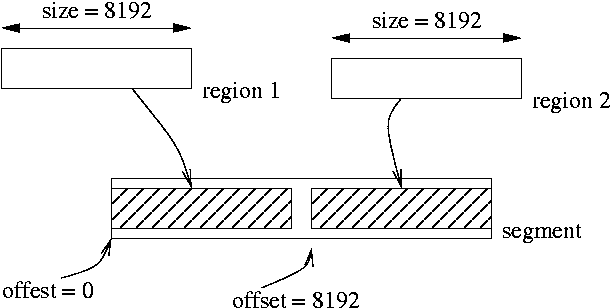
\includegraphics[width=0.4\linewidth]{figures/k1-offset}
  \end{center}

}

\function{t\_error}{region\_release}{\type{i\_as} \argument{asid},
				     \type{i\_region} \argument{regid}}
{
  This function releases the region \argument{regid} that belongs to the
  address space \argument{asid}.
}

\function{t\_error}{region\_inject}{\type{i\_as} \argument{asid},
                                    \type{o\_region*} \argument{o},
				    \type{i\_region*} \argument{regid}}
{
  This function injects the region \argument{o} into the address space
  \argument{asid}. 
}

\function{t\_error}{region\_flush}{\type{i\_as} \argument{asid}}
{
  This function releases all the regions of the address space \argument{asid}.
}

\function{t\_error}{region\_get}{\type{i\_as} \argument{asid},
				 \type{i\_region} \argument{regid},
				 \type{o\_region**} \argument{o}}
{
  This function returns the region object from its id \argument{regid} and the
  address space \argument{asid}, through the parameter \argument{o}.
}

\function{t\_error}{ia32\_pd\_activate}{\type{t\_ia32\_directory} \argument{dir},
                                        \type{t\_uint32} \argument{cached},
					\type{t\_uint32} \argument{writeback}}
{
  This function activates the page directory \argument{dir} by putting its
  address in the PDBR. The arguments \argument{cached} and \argument{writeback}
  control respectively if the cache should be enabled, or if the cache policy
  should be writeback. The flags of the PDBR register must be setup accordingly.
  
}

\function{t\_error}{ia32\_pd\_get\_cr3}{\type{t\_uint32*} \argument{cr3},
					\type{t\_ia32\_directory} \argument{dir},
					\type{t\_uint32} \argument{cached},
					\type{t\_uint32} \argument{writeback}}
{
  This function builds the value to put in the CR3 register to activate the page
  directory \argument{dir} with the \argument{cached} and \argument{writeback} flags
  set accordingly. The built value is returned in \argument{cr3}.
}

\function{t\_error}{ia32\_pd\_add\_table}{\type{t\_ia32\_directory*} \argument{dir},
					  \type{t\_uint16} \argument{entry},
					  \type{t\_ia32\_table} \argument{table}}
{
  This functions adds the page table \argument{table} in the page directory
  \argument{dir} at the index \argument{entry}.
}

\function{t\_error}{ia32\_pd\_get\_table}{\type{t\_ia32\_directory*} \argument{dir},
					  \type{t\_uint16} \argument{entry},
					  \type{t\_ia32\_table*} \argument{table}}
{
  This functions gets the page table \argument{table} from the page directory
  \argument{dir} at the index \argument{entry}.
}

\function{t\_error}{ia32\_pd\_delete\_table}{\type{t\_ia32\_directory*} \argument{dir},
					     \type{t\_uint16} \argument{entry}}
{
  This functions removes the page table at the index \argument{entry} from the
  page directory \argument{dir}.
}

\function{t\_error}{ia32\_pt\_build}{\type{t\_paddr} \argument{base},
				     \type{t\_ia32\_table*} \argument{table}}
{
  This function initializes the page table entry \argument{table} with the
  physical address \argument{base}
}

\function{t\_error}{ia32\_pt\_add\_page}{\type{t\_ia32\_table*} \argument{tab},
					 \type{t\_uint16} \argument{entry},
					 \type{t\_ia32\_page} \argument{page}}
{
  This functions adds the page \argument{page} in the page table
  \argument{tab} at the index \argument{entry}.
}

\function{t\_error}{ia32\_pt\_get\_page}{\type{t\_ia32\_table*} \argument{tab},
					 \type{t\_uint16} \argument{entry},
					 \type{t\_ia32\_page*} \argument{page}}
{
  This functions gets the page \argument{page} from the page table
  \argument{tab} at the index \argument{entry}.
}

\function{t\_error}{ia32\_pt\_delete\_page}{\type{t\_ia32\_table*} \argument{tab},
					    \type{t\_uint16} \argument{entry}}
{
  This functions removes the page at the index \argument{entry} from the
  page table \argument{tab}.
}

\function{t\_error}{ia32\_tlb\_invalidate}{\type{t\_vaddr} \argument{page}}
{
  This functions invalidates the TLB entry for the virual address
  \argument{page}.
}

\function{t\_error}{ia32\_tlb\_flush}{\type{void}}
{
  This functions flushes the TLB of the CPU.
}

\function{t\_error}{ia32\_map\_pd}{\type{t\_ia32\_directory*} \argument{pd}}
{
  This function takes the physical address of a page directory in \argument{pd}.
  It will map this page directory in the kernel address space, and return
  the virtual address by erasing the content of \argument{pd}.
  The type of the argument is a physical address, not a virtual address, but
  since they are both 32-bit values, you can just cast your virtual address
  to put it in the value pointed by \argument{pd}.
  In other words, when the function is called, it takes a physical address of
  a page directory in the memory space pointed by \argument{pd}, the function
  should then map this page directory, and the virtual address which has been
  assigned for this mapping should be put in the memory space pointed by
  \argument{pd} even though its type doesn't represent a virtual address.
}

\function{t\_error}{ia32\_map\_pt}{\type{t\_ia32\_table*} \argument{pt}}
{
  This function takes a page table structure in \argument{pt}. It will retrieve
  the physical address of this page from this struct, map it in the kernel address
  space, and return the virtual address through the appropriate field of this
  struct \argument{pt}.
}

\function{t\_error}{ia32\_map\_region}{\type{i\_as} \argument{asid},
                                       \type{i\_segment} \argument{segid},
				       \type{t\_paddr} \argument{offset},
				       \type{t\_opts} \argument{opts},
				       \type{t\_vaddr} \argument{address},
				       \type{t\_vsize} \argument{size}}
{
  This function will map the region defined by \argument{address} and \argument{size}
  on the segment defined by \argument{segid} at the offset \argument{offset}, in the
  address space defined by \argument{asid}.
  
  \-

  The \argument{opts} are similar to \emph{region\_reserve}.

  \-

  Refer to the figure in the \emph{region\_reserve} description to understand what
  \argument{offset} is used for.

  \-

  This function will create page tables if required.
}

\function{t\_error}{ia32\_unmap\_region}{\type{i\_as} \argument{asid},
					 \type{t\_vaddr} \argument{address},
					 \type{t\_vsize} \argument{size}}
{
  This function will unmap the region defined by \argument{address} and \argument{size}
  from the address space defined by \argument{asid}.

  \-

  This function must release the memory of page tables that gets empty upon unmapping.
}

\subsection*{Optional implementation}

The following functions are not going to be tested by our test suite, you are
not forced to do them although we strongly recommend you to do it, since they
are very helpful for debugging your implementation.

\-

Since this is not tested, the output format is up to you.

\function{t\_error}{region\_show}{\type{i\_as} \argument{asid},
                                  \type{i\_region} \argument{regid}}
{
  This function displays the region object specified by its id \argument{regid}
  and the address space \argument{asid}.
}

\function{t\_error}{region\_dump}{\type{i\_as} \argument{asid}}
{
  This function displays all the region objects that belong to the address
  space \argument{asid}.
}

\function{t\_error}{ia32\_pd\_dump}{\type{t\_ia32\_directory*} \argument{dir}}
{
  This function displays the content of the page directory \argument{dir}.
}

\function{t\_error}{ia32\_pt\_dump}{\type{t\_ia32\_pte*} \argument{tab}}
{
  This function displays the content of the page table \argument{dir}.
}

\subsection*{Important}
Please note that you have the core and the machine part to do.
All the functions might not require a machine part though. The machine
part file (glue) doesn't contain any prototypes.
It's your responsability to add a machine function, in glue if you think
it needs one.

\-

In the machine part, we also removed some full functions (including the prototypes). You are free to make new functions, to make your code cleaner, as long as you at least implement the required interface below.

\-

Some structures relative to the region manager are already provided, but you
are free to modify them if you want to. You can freely add new fields, and also
modify the existing ones, but in that case, it's your responsibility to make
changes in the code so that everything still works.

%%
%% licence       kaneton licence
%%
%% project       kaneton
%%
%% file          /home/mycure/kaneton/view/papers/assignments/k2.tex
%%
%% created       matthieu bucchianeri   [tue feb  7 11:49:56 2006]
%% updated       julien quintard   [fri mar  3 10:27:57 2006]
%%

%
% k2
%

\section{k2}

%
% informations
%

\subsection{Informations}

\begin{tabular}{p{7cm}l}
Deadline: & XXX, 23h42 \\
Duration: & two weeks \\
File name: & k1.tar.gz \\
In charge of: & Julien Quintard - \small{quinta\_j@epita.fr} \\
Newsgroups: & epita.kaneton \\
Languages: & Assembly and C \\
Architectures: & Intel Architecture 32-bit \\
Students per group: & three \\
\end{tabular}

%
% overview
%

\subsection{Overview}

The \textbf{k2} project consists in the development of parts of
the kaneton core including:

\begin{itemize}
  \item
    The id manager.
  \item
    The set manager.
  \item
    The address space manager.
  \item
    The segment manager.
\end{itemize}

XXX

%
% assignments
%

\subsection{Assignments}

%
% id manager
%

\subsubsection{id manager}

The id manager is very important because it is very simple and will
introduce you how managers are implemented in kaneton.

Every student should be able to understand it before starting other
managers.

The id manager is used to generate unique identifiers from an identifier
object.

Once the identifier object initialised, you can use your
identifier object \textbf{o\_id} to generate unique identifiers.

Remember that, in the current kaneton implementation, identifiers only
consist in 64-bit integers. Therefore, the id manager does not take care
of identifiers recycling.

Now, let's take a look at the id manager functions you will implement:

\prototype{t\_error \textbf{id\_show}(o\_id* \textit{o});}

This function just displays an id object's state.

\prototype{t\_error \textbf{id\_clone}(o\_id* \textit{o},
                                       t\_id \textit{old},
                                       t\_id* \textit{new});}

This function duplicates an id object using the \textit{o} identifier
object.

\prototype{t\_error \textbf{id\_reserve}(o\_id* \textit{o},
                                         t\_id* \textit{u});}

This function reserves an identifier \textit{u} using the identifier
object \textit{o}.

\prototype{t\_error \textbf{id\_release}(o\_id* \textit{o},
                                         t\_id \textit{u});}

This function releases the identifier \textit{u}.

\prototype{t\_error \textbf{id\_build}(o\_id* \textit{o});}

This function initializes an identifier object.

\prototype{t\_error \textbf{id\_destroy}(o\_id* \textit{o});}

This function destroys an identifier object.

\prototype{t\_error \textbf{id\_init}(void);}

This function just initializes the id manager.

\prototype{t\_error \textbf{id\_clean}(void);}

This function just cleans the id manager.

Like every other managers in kaneton, the \textbf{id\_init()} and
\textbf{id\_clean()} functions must be called by the kernel main
routine on startup and shutdown.

%
% set manager
%

\subsubsection{set manager}







----------------------------------------------------------------------

as  and  segment  introduce  calls  to  machine-dependent  code,  this
mecanism  must be well  understood by  every students.  Moreover, many
parts of  the kernel will  lead student to  use the sets, so  the sets
interface must be clearly understood.

For the two first managers,  you have to follow precisely the bevavior
as described  in the kaneton  reference documentation. For  the memory
management, you must be totally compliant with the given interface and
the   described   behavior,   but   algorithm  (especially   for   the
machine-dependent code) are design-free.

To  finish, notice  that  the current  implementation  of the  console
driver is not clean and will be changed in future kaneton projects.

%
% id manager
%

%
% set manager
%

\subsection{set manager}

\subsubsection{Description}

The set  manager is used to  store data. Every kernel  managers use it
instead of building data structures by their own.

The set mecanism is divided in  two parts: the set manager and the set
implementations.

While the set implementations are specific to each type of set (array,
linked-list\ldots), the set manager code  is generic and work with all
sets.

\subsubsection{Students work}

The  manager code  is given,  see  \textit{core/kaneton/set/set.c} and
\textit{core/include/kaneton/set.h}.  Take a  look at  the information
section in the header of the  manager code: each steps of the creation
of a set is described.

The student will have to  write the entire code for the \textbf{array}
and \textbf{ll} implementations.

The functions below are explained independently of the data structure.

\prototype{t\_error \textbf{set\_type\_[x]}(t\_setid \textbf{setid});}

This function just returns an error if the set corresponding to
\textbf{setid} is not of the type \textbf{[x]}.

\prototype{t\_error \textbf{set\_show\_[x]}(t\_setid \textbf{setid});}

This function displays a entire set.

\prototype{t\_error \textbf{set\_head\_[x]}(t\_setid \textbf{setid},
                                            t\_iterator* \textbf{iterator});}

This function returns an iterator on the first element of the set.

\prototype{t\_error \textbf{set\_tail\_[x]}(t\_setid \textbf{setid},
                                            t\_iterator* \textbf{iterator});}

This function returns an iterator on the last element of the set.

\prototype{t\_error \textbf{set\_prev\_[x]}(t\_setid \textbf{setid},
                                            t\_iterator \textbf{current},
                                            t\_iterator* \textbf{previous});}

This function returns an iterator on the previous element of the set.

\prototype{t\_error \textbf{set\_next\_[x]}(t\_setid \textbf{setid},
                                            t\_iterator \textbf{current},
                                            t\_iterator* \textbf{previous});}

This function returns an iterator on the next element of the set.

\prototype{t\_error \textbf{set\_insert\_head\_[x]}(t\_setid \textbf{setid},
                                                    void* \textbf{data});}

This function inserts an object at the head of the set.

\prototype{t\_error \textbf{set\_insert\_tail\_[x]}(t\_setid \textbf{setid},
                                                    void* \textbf{data});}

This function inserts an object at the tail of the set.

\prototype{t\_error \textbf{set\_insert\_before\_[x]}(t\_setid \textbf{setid},
                                                      t\_iterator \textbf{iterator},
                                                      void* \textbf{data});}

This function inserts an object before the one specified by the iterator.

\prototype{t\_error \textbf{set\_insert\_after\_[x]}(t\_setid \textbf{setid},
                                                     t\_iterator \textbf{iterator},
                                                     void* \textbf{data});}

This function inserts an object after the one specified by the iterator.

\prototype{t\_error \textbf{set\_add\_[x]}(t\_setid \textbf{setid},
                                           void* \textbf{data});}

This function adds an object in the set. See at the end of the section
for more details.

\prototype{t\_error \textbf{set\_remove\_[x]}(t\_setid \textbf{setid},
                                              t\_id \textbf{id});}

This function removes an object identified by \textbf{id} from the
set \textbf{setid}.

\prototype{t\_error \textbf{set\_delete\_[x]}(t\_setid \textbf{setid},
                                              t\_iterator \textbf{iterator});}

This function deletes the object corresponding to the iterator.

\prototype{t\_error \textbf{set\_flush\_[x]}(t\_setid \textbf{setid});}

This function removes every object stored in the set.

\prototype{t\_error \textbf{set\_locate\_[x]}(t\_setid \textbf{setid},
                                              t\_id \textbf{id},
                                              t\_iterator* \textbf{iterator});}

This function returns an iterator on the element corresponding to the
identifier \textbf{id}.

\prototype{t\_error \textbf{set\_object\_[x]}(t\_setid \textbf{setid},
                                              t\_iterator \textbf{iterator},
                                              void** \textbf{data});}

This function returns the object's data corresponding to the iterator.

\prototype{t\_error \textbf{set\_push\_array}(t\_setid \textbf{setid},
                                             void* \textbf{data});}

This function adds an object to a FIFO or LIFO structure.

\prototype{t\_error \textbf{set\_pop\_array}(t\_setid \textbf{setid});}

This function removes the next object of a FIFO or LIFO structure.

\prototype{t\_error \textbf{set\_pick\_array}(t\_setid \textbf{setid},
                                             void** \textbf{data});}

This  function returns the  next object  of a  FIFO or  LIFO structure
without deleting it.

\prototype{t\_error \textbf{set\_release\_[x]}(t\_setid \textbf{setid});}

This function releases a set.

The two last functions are  described more specificaly since they have
different prototypes.

\prototype{t\_error \textbf{set\_reserve\_ll}(t\_opts \textbf{opts},
                                              t\_size \textbf{datasz},
                                              t\_setid* \textbf{setid});}

This function reserves a ll set with options \textbf{opts} which will contain
object of \textbf{datasz} size.

\prototype{t\_error \textbf{set\_reserve\_array}(t\_opts \textbf{opts},
                                                 t\_setsz \textbf{initsz},
                                                 t\_size \textbf{datasz},
                                                 t\_setid* \textbf{setid});}

This function reserves an array set with options \textbf{opts}. This
set will contain objects of \textbf{datasz} size and will initialy
be composed of \textbf{initsz} unused elements.

You can notice  that some operations does not make  sense on some data
structures. For  example, \textbf{push} or \textbf{pop}  will never be
used on arrays or lists, but  only on stacks or pipes. In these cases,
the function must be present but will only return an error.

Most   widely,    some   operations   have   no    sense   with   some
options. Inserting at the beginning  of a sorted array must produce an
error since it can cancel the sorting property.

\subsubsection{Constraints}

To  keep  sets behavior  unified,  here  are  some rules  applying  to
\textbf{array} and \textbf{ll}:

\begin{itemize}

\item \textbf{set\_add\_array} must insert the item at the first free place.

\item All deletion functions on arrays must mark the released place as
free. The only case shifting is made is when the \textbf{organise} option
is set.

\item When inserting an object in a linked-list with the \textbf{add}
operation, the item must be placed in the head of the list.

\item As double linked-list are faster than simple one, you have to
implement this kind of lists.

\end{itemize}

Here are the options your sets must recognize:

\begin{itemize}
\item SET\_OPT\_CONTAINER
\item SET\_OPT\_ALLOC and SET\_OPT\_FREE
\item SET\_OPT\_SORT
\item SET\_OPT\_ORGANISE (for arrays only)
\end{itemize}

Do  not  forget to  uncomment  the  step  5 of  \textbf{set\_init}  in
\textit{core/kaneton/set/set.c}, which creates the set container.

%
% address space manager
%

\subsection{address space manager}

\subsubsection{Description}

The address space manager just  manages the address spaces. An address
space is a container describing the addressable memory.

An address space is composed of a set of segments and a set of regions.

\subsubsection{Students work}

Students have to write the whole  code of this manager. No need to say
that intensive use of  sets (previously described) is necessary.  This
manager will introduce you how to program with the set manager.

\prototype{t\_error \textbf{as\_show}(t\_asid \textbf{asid});}

This function shows a precise address space displaying information
on it.

\prototype{t\_error \textbf{as\_dump}(void);}

This function dumps all the address space managed by the address
space manager.

\prototype{t\_error \textbf{as\_clone}(t\_tskid \textbf{tskid},
                                       t\_asid \textbf{old},
                                       t\_asid* \textbf{new});}

This function clones an address space taking care of cloning everything
necessary.

\prototype{t\_error \textbf{as\_reserve}(t\_tskid \textbf{tskid},
                                         t\_asid* \textbf{asid});}

This  function   reserves  an  address  space  object   for  the  task
\textbf{tskid}. For k2, you don't have to deal with tasks, so you must
ignore \textbf{tskid}.

\prototype{t\_error \textbf{as\_release}(t\_asid \textbf{asid});}

This function just  releases an address space.

\prototype{t\_error \textbf{as\_get}(t\_asid \textbf{asid},
                                    o\_as** \textbf{o});}

This function should only be used by the segment and region managers.

This function just returns the address space object corresponding to
the address space identifier.

\prototype{t\_error \textbf{as\_init}(void);}

This function initialises the address space manager.

\prototype{t\_error \textbf{as\_clean}(void);}

This function cleans the address space manager.

%
% ia32
%

\subsubsection{IA-32 implementation}

Students will  have to develop the architecture-dependent  part of the
address space manager.

The corresponding file is \textit{core/kaneton/arch/\textbf{arch-name}/as.c}.

Students have  to think about what  is an address space  from the ia32
point of view.  Next, they will fill the \textbf{do\_as} structure in
\textit{core/include/arch/\textbf{arch-name}/kaneton/as.h}

To  finish,   they  must   implement  all  dependent   functions  they
need. Remember that functions in \textit{libia32} should be reused.

Take a look at the  kaneton reference paper for more information about
machine-dependent calls.

%
% segment manager.
%

\subsection{segment manager}

\subsubsection{Description}

The segment manager manages physical  memory. Its goals are to reserve
and release physical pages, merge or split allocated pages and finally
to read or write directly into physical memory.

\subsubsection{Students work}

Students have to write everything in this manager. Some functions will
be added in k3.

\prototype{t\_error \textbf{segment\_show}(t\_segid \textbf{segid});}

This function displays information on specified segment.

\prototype{t\_error \textbf{segment\_dump}(void);}

This function displays all segments in the segment container.

\prototype{t\_error \textbf{segment\_clone}(t\_asid \textbf{asid},
                                            t\_segid \textbf{old},
                                            t\_segid* \textbf{new});}

This function clones a segment copying its content.

\prototype{t\_error \textbf{segment\_inject}(o\_segment* \textbf{seg},
                                             t\_asid \textbf{asid});}

This  function   injects  a  pre-allocated  segment   in  the  segment
container.  This function  concerns k1  pre-reserved segments.  All of
these must be passed to the inject function at kernel boot time.

\prototype{t\_error \textbf{segment\_give}(t\_asid \textbf{asid},
                                           t\_segid \textbf{segid});}

This function gives an address space from one process to another.

\prototype{t\_error \textbf{segment\_resize}(t\_segid \textbf{segid},
                                             t\_psize \textbf{new\_size},
                                             t\_segid \textbf{new\_seg});}

This function resizes a segment.

\prototype{t\_error \textbf{segment\_split}(t\_segid \textbf{segid},
                                            t\_psize \textbf{sz1},
                                            t\_segid* \textbf{s1},
                                            t\_segid* \textbf{s2});}

This function split a segment into two segments.

\prototype{t\_error \textbf{segment\_coalesce}(t\_segid \textbf{s1},
                                               t\_segid \textbf{s2},
                                               t\_segid* \textbf{new\_seg});}

This function merges two segments into a single one.

\prototype{t\_error \textbf{segment\_reserve}(t\_asid \textbf{asid},
                                              t\_psize \textbf{size},
                                              t\_perms \textbf{perms},
                                              t\_segid* \textbf{segid});}

This function reserves a segment of specified size.

\prototype{t\_error \textbf{segment\_release}(t\_segid \textbf{segid});}

This function releases a segment.

\prototype{t\_error \textbf{segment\_catch}(t\_asid \textbf{asid},
                                            t\_segid \textbf{segid});}

This function  is used to  force a segment  to be given to  an address
space.  ``catcheable''  segments  are   reserved  by  the  kernel  for
architecture specific managers. Catcheable segments are defined in the
\textit{kaneton.conf} file.

\prototype{t\_error \textbf{segment\_perms}(t\_segid \textbf{segid},
                                            t\_perms \textbf{perms});}

This function changes permissions for a segment.

\prototype{t\_error \textbf{segment\_type}(t\_segid \textbf{segid},
                                           t\_type \textbf{type});}

This function retrieves the type of a segment.

\prototype{t\_error \textbf{segment\_flush}(t\_asid \textbf{asid});}

This function  flushes the  segment container, releasing  all segments
for all address spaces.

\prototype{t\_error \textbf{segment\_get}(t\_segid \textbf{segid},
                                          o\_segment** \textbf{o});}

This  function  gets  the  segment  object  associated  to  a  segment
identifier.

\prototype{t\_error \textbf{segment\_init}(void);}

This function initialises the segment manager.

\prototype{t\_error \textbf{segment\_clean}(void);}

This function cleans the segment manager.

In  addition,  students  have  to  implement  a  first-fit  allocation
algorithm for physical pages.

\prototype{t\_error \textbf{segment\_fit}(o\_as* \textbf{as},
                                          t\_psize \textbf{size},
                                          t\_paddr* \textbf{address});}

This function searchs  the given address space for  a segment of given
size.

This function must  be placed in a separated file: take  a look at the
\textbf{\_SEGMENT\_FILE\_} variable in you \textit{user.conf} file.

As there  can be more than  one algorithm available, do  not forget to
use  the  \textbf{SEGMENT\_FIT} define  in  your \textit{conf.h}  file
(default  value is \textbf{FIT\_FIRST}.  More values  can be  added in
\textit{core/include/kaneton/kaneton.h}

\subsubsection{IA-32 implementation}

Students  have to  implement all  the architecture-dependent  code for
Intel.

Depending  on the  chosen variation  around IA-32,  there  are several
rules to follow:

\begin{itemize}

\item ia32-virtual:
\begin{itemize}

\item Segment  sizes are  aligned on page  size. Assuming you  are not
using PSE  (4 Mbyte pages), this  value will be 4096.  Remember to use
the \textbf{PAGESZ} define.

\item You must create two segments  (one for code, the other for data)
per task class:  kernel, driver, service, and user  program.  Each one
must have the appropriate privilege level and permissions.

\end{itemize}

\item ia32-segment:
\begin{itemize}

\item Obi-Wan Kenobi

\end{itemize}
\end{itemize}

%
% console manager
%

\subsection{console manager}

\subsubsection{Students work}

In fact only two functions are required for the console driver.

\prototype{void \textbf{cons\_attr}(t\_uint8 \textbf{attr});}

This is  the first \textbf{required} function.  This function modifies
display attributes for next characters printing.

\prototype{int \textbf{cons\_print\_char}(char \textbf{c});}

This  is  the second  \textbf{required}  function.  It  adds a  single
character with the currently defined attribute.

Next  functions   are  not  necessary,  but  you   must  provide  some
equivalent.

\prototype{void \textbf{cons\_clear}(void);}

This function clears the console.

\prototype{void \textbf{cons\_scroll}(t\_uint16 \textbf{lines});}

This function scrolls by given number of lines.

\prototype{void \textbf{cons\_print\_string}(char* \textbf{string});}

This function prints a string.

\prototype{void \textbf{cons\_msg}(char \textbf{indicator},
                                   char* \textbf{fmt},
                                   ...);}

This function is used to display formatted and coloured messages.

\prototype{t\_error \textbf{cons\_init}(void);}

\prototype{t\_error \textbf{cons\_clean}(void);}

%
% klibc introduction
%

\subsection{klibc introduction}

%
% modification to kernel main
%

\subsection{kernel main procedure}

As the first managers are now  working, it is time to write the kernel
main procedure.

This  one is  contained  in \textit{core/kaneton/kaneton.c}.  Students
must first initialize the \textbf{init} variable from the one given by
the bootloader. Then, they  must initialize the differents manager. Do
not forget that  it is better to initialize the  set manager before as
and segment, since these managers rely on sets !

Do not  forget to  initialize the kernel  standard library.   You must
initialize  the  \textbf{printf}  function  passing  pointers  to  the
console  manager functions to  \textbf{print\_init}. In  addition, you
must initialize the kernel  \textbf{malloc} function which is used for
early initial stages  (until as, segment and region  are running, this
will  be  possible  in  k3).  You must  use  the  \textbf{alloc\_init}
function,  passing  the  survival   area  pre-allocated  in  k1  (fields
\textbf{alloc} and \textbf{allocsz} of \textbf{t\_init}).

To finish, you  have to create the kernel address  space and to inject
the pre-allocated segments in.

Finally, all  managers must be destroyed  calling the \textbf{\_clean}
functions for each one (in the good order !).

You might place  code for your tests between these  two phases. Do not
forget to disable it for the final tarball.

%
% bonus
%

\subsection{k2 bonus}

Students can implement a better allocation algorithm for
segments, like Buddy systems.


XXX expliquer lorsqu'on aborde les sets que vu que ca se base sur
XXX malloc il fallait trouver une solution


%%
% ---------- header -----------------------------------------------------------
%
% project       kaneton
%
% license       kaneton
%
% file          /home/mycure/kaneton/view/talk/presentations/k3/k3.tex
%
% created       julien quintard   [sat nov 29 20:40:35 2008]
% updated       julien quintard   [fri apr 10 02:01:41 2009]
%

%
% ---------- setup ------------------------------------------------------------
%

%
% path
%

\def\path{../../..}

%
% template
%

%
% ---------- header -----------------------------------------------------------
%
% project       kaneton
%
% license       kaneton
%
% file          /home/mycure/kaneton/view/template/lecture.tex
%
% created       julien quintard   [wed may 16 18:17:26 2007]
% updated       julien quintard   [sun may 18 23:23:40 2008]
%

%
% class
%

\documentclass[8pt]{beamer}

%
% packages
%

\usepackage{pgf,pgfarrows,pgfnodes,pgfautomata,pgfheaps,pgfshade}
\usepackage[T1]{fontenc}
\usepackage{colortbl}
\usepackage{times}
\usepackage{amsmath,amssymb}
\usepackage{graphics}
\usepackage{graphicx}
\usepackage{color}
\usepackage{xcolor}
\usepackage[english]{babel}
\usepackage{enumerate}
\usepackage[latin1]{inputenc}
\usepackage{verbatim}
\usepackage{aeguill}

%
% style
%

\usepackage{beamerthemesplit}
\setbeamercovered{dynamic}

%
% verbatim stuff
%

\definecolor{verbatimcolor}{rgb}{0.00,0.40,0.00}

\makeatletter

\renewcommand{\verbatim@font}
  {\ttfamily\footnotesize\selectfont}

\def\verbatim@processline{
  {\color{verbatimcolor}\the\verbatim@line}\par
}

\makeatother

%
% -
%

\renewcommand{\-}{\vspace{0.4cm}}

%
% date
%

\date{\today}

%
% logos
%

\pgfdeclareimage[interpolate=true,width=34pt,height=18pt]
                {epita}{\path/logo/epita}
\pgfdeclareimage[interpolate=true,width=49pt,height=18pt]
                {upmc}{\path/logo/upmc}
\pgfdeclareimage[interpolate=true,width=25pt,height=18pt]
                {lse}{\path/logo/lse}

\newcommand{\logos}
  {
    \pgfuseimage{epita}
  }

%
% institute
%

\institute
{
  \inst{1} kaneton microkernel project
}

%
% table of contents at the beginning of each section
%

\AtBeginSection[]
{
  \begin{frame}<beamer>
   \frametitle{Outline}
    \tableofcontents[current]
  \end{frame}
}

%
% table of contents at the beginning of each subsection
%

\AtBeginSubsection[]
{
  \begin{frame}<beamer>
   \frametitle{Outline}
    \tableofcontents[current,currentsubsection]
  \end{frame}
}


%
% title
%

\title{k3}

%
% document
%

\begin{document}

%
% title frame
%

\begin{frame}
  \titlepage
\end{frame}

%
% outline frame
%

\begin{frame}
  \frametitle{Outline}

  \tableofcontents
\end{frame}

%
% ---------- text -------------------------------------------------------------
%

%
% introduction
%

\section{Introduction}

% 1)

\begin{frame}
  \frametitle{Overview}

  \name{k3} is a stage that can be considered as \term{open}.

  \-

  Indeed, total freedom is given to students regarding the design and
  implementation of this project.
\end{frame}

% 2)

\begin{frame}
  \frametitle{Objective}

  The goal of this project is for students to design and implement the
  feature of their choice.
\end{frame}

%
% assignments
%

\section{Assignments}

% 1)

\begin{frame}
  \frametitle{Design}

  The first task consists for students to design the system by studying
  the different algorithms and techniques.
\end{frame}

% 2)

\begin{frame}
  \frametitle{Interface}

  The students feature is not meant to comply to any pre-defined interface.

  \-

  As such, students are invited to study the limitations of well-known
  interfaces such as \name{POSIX}'s in order to define a new one. Additional
  points will be granted according to the solution they propose.
\end{frame}

% 3)

\begin{frame}
  \frametitle{Implementation}

  Once the system designed, students will have to implement it by
  taking care of providing a few illustrating applications.

  \-

  Indeed, no test application is provided as total freedom is given to
  students regarding the interface.
\end{frame}

%
% evaluation
%

\section{Evaluation}

% 1)

\begin{frame}
  \frametitle{Viva}

  During the viva, students will have to first describe their choices in
  terms of design before detailling what problems they encountered afterwards
  regarding the previously sketched design.

  \-

  The services interface and user-level applications should also be discussed,
  though quite briefly.

  \-

  The viva will last for $10$ minutes with possibly $5$ minutes for questions.
\end{frame}

%
% conclusion
%

\section{Conclusion}

% 1)

\begin{frame}
  \frametitle{Freedom}

  The main objective of this stage is to give students total control over
  a well-defined functionality.

  \-

  Students should therefore take advantage of this freedom to study and
  think about what well-known systems provide and whether such systems are
  actually good or bad.
\end{frame}

%
% bibliography
%

\begin{frame}
  \frametitle{Bibliography}

  \bibliographystyle{amsplain}
  \bibliography{\path/bibliography/bibliography}
\end{frame}

\end{document}


%%%
%% copyright quintard julien
%% 
%% kaneton
%% 
%% k4.tex
%% 
%% path          /root/data/research/projects/svn/kaneton/notes/k4
%% 
%% made by mycure
%%         quintard julien   [quinta_j@epita.fr]
%% 
%% started on    Mon Mar 21 13:16:44 2005   mycure
%% last update   Mon Mar 21 13:18:10 2005   mycure
%%

\documentclass[10pt,a4wide]{article}
\usepackage[english]{babel}
\usepackage{a4wide}
\usepackage{graphicx}
\usepackage{graphics}
\usepackage{fancyheadings}
\pagestyle{fancy}

\bibliographystyle{plain}

\lhead{{\scriptsize kaneton project}}
\rhead{k4 notes}
\rfoot{\scriptsize EPITA System Lab}

\title{k4}

\author{Julien Quintard - \small{quinta\_j@epita.fr} \\
        Jean-Pascal Billaud - \small{billau\_j@epita.fr} \\ \\
	\small{last updated by} \\
	Julien Quintard - \small{quinta\_j@epita.fr}}

\date{\today}

\begin{document}
\maketitle

\section{Notes}

\begin{enumerate}

\item explication g\'en\'erale du projet

\item explication des interfaces

\item scheduler:

\begin{verbatim}

(*) le kernel doit garder en memoire:
	. a) le nombre de processes en cours
	. b) la somme des priorites des processes
	. c) le quantum actuel

	-> quantum total = a * c
	-> quantum du process = priority * quantum total / b

(*) le process doit garder en memoire:
        . d) le nombre de threads
	. e) la somme des priorites des threads

	-> quantum du thread = priority * quantum du process / e

(*) si le quantum d'un process descend en dessous du seuil de la classe
    inferieure c'est que ca commence a devenir tendu et la par exemple
    on pourrait envisager sur un systeme distribue a migrer des processus
    et a lancer les nouveaux processus sur une autre machine.

\end{verbatim}

exemple:

\begin{verbatim}

5 tasks avec une somme de priorites de 276 avec 20ms par defaut par processus
soit 20*5=100ms pour tout le monde:
        1) B 15
        2) R 100
        3) T 33
        4) T 58
        5) I 70

IL FAUT DONC TJS GARDER LA SOMME DES PRIORITES DES PROCESSUS

1) 15*100/276   =       5.4             /* a calculer en ticks apres */
2) 100*100/276  =       36.2
3) 33*100/276   =       11.9
4) 58*100/276   =       21.0
5) 70*100/276   =       25.3

                        99.8

\end{verbatim}

\end{enumerate}

\end{document}


\end{document}
